% ********** Chapter 1 **********
\section{Design}
\label{sec:chap1:design}

Eine JSR 223 Implementation f"ur PHP besteht gezwungenermassen aus zwei Teilen: einem Java-Teil, welcher im Wesentlichen
die ScriptEngineFactory enth"alt, komplett in Java ohne die Verwendung von nativen (JNI-) Aufrufen implementiert ist und
s"amtliche Funktionalit"at des Auffindungsmechanismus abdeckt, sowie einem nativen Teil, welcher aus 
einem C- oder C++ - Programm, das die n"otigen Aufrufe an PHP vornimmt besteht.
Die eigentliche ScriptEngine verbindet diese beiden Teile indem sie aus Java heraus dieses, in nativen Code "ubersetzte, 
Programm mittels JNI anspricht.
Um allerdings JSR 223 "uberhaupt nutzen zu k"onnen m"ussen die Klassen aus javax.script, vor allem der ScriptEngineManager, 
im Java-Classpath liegen. Hierzu kann entweder eine Java-Runtime der Version 6, oder aber eine eigene Implementation dieser
Klassen genutzt werden. 
Die im folgenden beschriebene JSR 223 Implementation tr"agt den Namen "'Turpitude"'.

\subsection{Java}
\label{sec:chap1:design:java}

Um f"ur den ScriptEngineManager auffindbar zu sein muss eine JSR 223 Implementation sich gem"ass der \emph{Jar File Specification} \cite{JARSPEC} 
als sogenannter \emph{Service Provider} registrieren. Hierzu muss sich im Verzeichnis \emph{META-INF/services} des .jars eine Datei
mit dem Namen der Service-Klasse (in diesem Fall \emph{javax.script.ScriptEngineFactory}) befinden, in welcher verf"ugbare 
ScriptEngineFactories zeilenweise aufgelistet werden.

Alle Klassen der Implementation befinden sich im Package \emph{net.xp\_framework.turpitude}. 
Die ScriptEngineFactory-Implementation hei\ss t \emph{PHPScriptEngineFactory} und implementiert direkt das Interface 
\emph{ScriptEngineFactory} aus \emph{javax.script}. Im Gegensatz dazu implementiert die Klasse \emph{PHPScriptEngine} nicht
direkt das Interface \emph{ScriptEngine}, sondern erbt von der abstrakten Klasse \emph{AbstractScriptEngine}, welche f"ur
viele Varianten der \emph{eval()}-Methode schon eine Realisierung, sowie mit der Klasse \emph{SimpleScriptContext} schon einen 
\emph{ScriptContext} mitbringt. Um den "ubergebenen Scriptcode tats"achlich auszu"fuhren muss dieser an den mittels der Java-Methode
\emph{System.loadLibary()} geladenen nativen Teil der Implementation weitergegeben werden. Die Kommunikation mit diesem
nativen Teil findet mittels JNI-Methoden statt.
Weiterhin implementiert die PHPScriptEngine die beiden in \emph{javax.script} enthaltenen Interfaces \emph{Compilable} und
\emph{Invocable}, deren Funktionalit"at zur Erff"ullung einiger der Use-Cases ben"otigt wird. F"ur die Methoden aus
Compilable wird noch eine weitere Klasse - \emph{PHPCompiledScript} - erstellt, welche direkt von der abstrakten
Klasse \emph{javax.script.CompiledScript} erbt.
Der Standard schrwibt zwar vor dass die ScriptEngine das Interface Invocable implementiert, allerdings ergibt das aus Sicht
des Autors nur wenig Sinn - auf welchem Script sollen Methoden und Funktionen aufgerufen werden? Auf dem zuletzt ausgef"uhrten?
Was wenn noch kein Script ausgef"uhrt wurde? Aus diesem Grund wird auch das PHPCompiledScript dieses Interface implementieren,
und Aufrufe der Interfacemethoden bei der PHPScriptEngine werden an das zuletzt "ubersetzte Script weitergeleitet.

Die Kommunikation zwischen Java und PHP findet "uber zwei unterschiedliche Kan"ale statt:

Bei der R"uckgabe von Daten aus einem PHP-Skript werden diese einfach kopiert, wobei simple Datentypen (bool, long, double und string)
einfach in ihre Java-"Aquivalente (java.lang.Boolean, java.lang.Long, java.lang.Double und java.lang.String) umgesetzt werden.
Da alle Arrays in PHP assoziativer Natur sind werden sie als untypisierte java.util.HashMap, das heisst sowohl der Schl"ussel als auch der Wert
sind vom Typ java.lang.Object, zur"uckgegeben. Einzig f"ur PHP-Objekte wird eine gesonderte Java-Klasse ben"otigt: \emph{PHPObject} enth"alt neben
der Klassennamen auch alle Eigenschaften eines PHP-Objektes. Diese werden in einer HashMap gespeichert, mit dem Namen der Eigenschaft
als Schl"ussel.
\begin{floatingtable}{
\label{tab:javatophp}
\begin{tabular}{|l|l|}
\hline
Java-Typ & PHP-Typ\\
\hline\hline
jlong & long\\
jint & long\\
jshort & long\\
jchar & long\\
jbyte & long\\
jboolean & bool\\
jfloat & double\\
jdouble & double\\
jstring & string\\
jobject & TurpitudeJavaObject\\
jclass & TurpitudeJavaClass\\
type[] & TurpitudeJavaArray\\
\hline
\end{tabular}}
\caption{\textsc{Java nach PHP}}
\end{floatingtable}
Leider h"alt sich die JSR223-Spezifikation zu vielen Fragen sehr bedeckt, so wird beispielsweise zur Typkonversion nur lapidar auf 
"'Implementationsdetails"' verwiesen. Da der Datenaustausch zwischen PHP und Java allerdings einen nicht unwesentlichen Bestandteil
einer JSR223-Implemenation darstellt, muss wohl oder "ubel eine Konvention gefunden werden. Die Tabellen \ref{tab:javatophp} und \ref{tab:phptojava}
erl"autern diese Konvetion, sowohl von Java nach PHP als auch umgekehrt. Weiterhin wird bei der Typkonversion von PHP nach Java zwischen 
Methodenaufrufen und Werter"uckgaben unterschieden. Bei Methodenaufrufen wird versucht in simple Datantypen wie \emph{int} und \emph{double}
umzuwandeln, weil der Standard oft aber verlangt dass Objekte zur"uckgegeben werden wird bei der R"uckgabe von Werten in den entsprechenden
Objektyp wie \emph{java.lang.Boolean} konvertiert. Einige Java-Klassen und PHP-Objekte werden speziell konvertiert, so wird beispielsweise
der java.lang.String nicht zu einem TurpitudeJavaObject, sondern zu einem String in PHP, diese F"alle sind gesondert aufgef"uhrt. Die
Tabellen enthalten auch Verweise auf spezielle PHP-Klassen, die sp"ater im Kapitel \ref{sec:chap1:design:native} erl"autert werden.

\begin{table}
\label{tab:phptojava}
\caption{\textsc{PHP nach Java, Methodenaufruf und Werter"uckgabe}}
\begin{tabular}[tbh]{|l|l|l|}
\hline
PHP-Typ & Methodenaufruf & Werter"uckgabe\\
\hline\hline
long & jlong & java.lang.Long \\
double & jdouble & java.lang.Double \\
bool & jboolean  & java.lang.Boolean \\
array & java.util.HashTable & java.util.HashTable \\
object & PHPObject & PHPObject\\
constant & jstring & jstring\\
string & jstring & jstring \\
TurpitudeJavaClass & jclass & jstring\\
TurpitudeJavaObject & jobject & jobject\\
TurpitudeJavaArray & jarray & jarray\\
\hline
\end{tabular}
\end{table}


Die Eingabe von Daten aus Java heraus in ein PHP-Skript geschieht - gem"a\ss der JSR223-Spezifikation - mittels des Kontextes der
ScriptEngine. Hierzu wird dieser - zusammen mit einigen Umgebungsvariablen und -Informationen - in eine globale Variable injiziert,
deren Name sich in der ScriptEngine setzen l"asst. Im Unterschied zu den oben beschriebenen R"uckgabewerten stellen die Kontext-Objekte
Referenzen dar, so wirken sich "Anderungen an diesen unmittelbar auf die entsprechenden Java-Objekte aus.

Die Abbildung \ref{fig:jsr223impl} zeigt die beteiligten Klassen und ihre Abh"anigkeiten untereinander,
zusammen mit einigen wichtigen Methoden und Attributen. 

\begin{figure}[h]
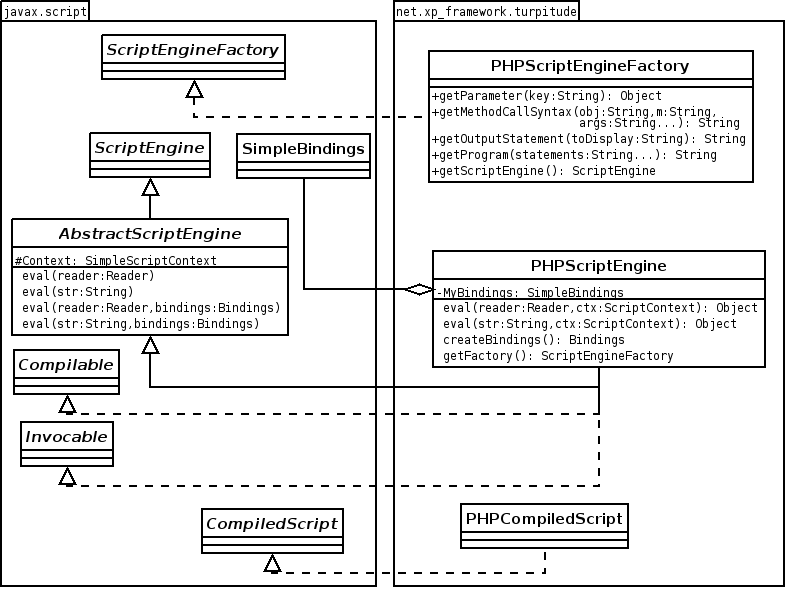
\includegraphics[width=\textwidth]{chap1/img/turpitude.png}
\caption{JSR 223 Implementation - Architektur}
\label{fig:jsr223impl}
\end{figure}

Der JSR 223 spezifiziert nur eine Exception (\emph{javax.script.ScriptException}) um alle m"oglichen Laufzeitfehler innerhalb einer 
Implementation abzudecken. Um dem Anwender trotzdem eine M"oglichkeit einer differenzierten Fehlerauswertung zu geben werden drei
zus"atzliche Exceptions eingef"uhrt: \emph{PHPScriptException}, \emph{PHPCompileException} und \emph{PHPEvalException} (siehe Abbildung
\ref{fig:jsr223exceptions}). Die PHPScriptException dient zum Einen als Oberklasse, zum anderen kann der Anwender durch sie erkennen, ob
das aufgetretene Problem implementationsspezifisch ist. Die beiden anderen neuen Exceptions werden genutzt um Fehler beim "Ubersetzen 
(PHPCompileException) oder beim Ausf"uhren (PHPEvalException) eines Skriptes voneinander abzugrenzen.

\begin{figure}[h]
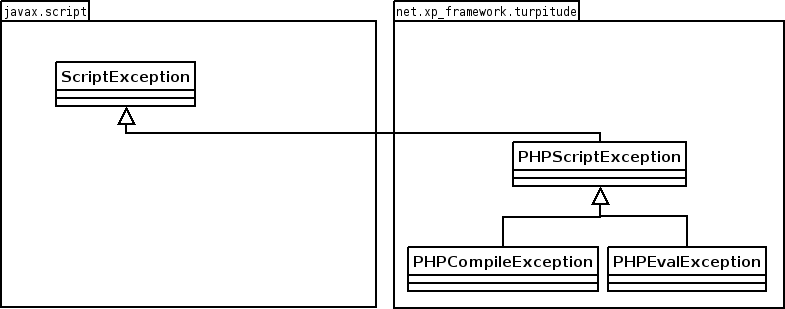
\includegraphics[width=\textwidth]{chap1/img/exceptions.png}
\caption{JSR 223 Implementation - Exceptions}
\label{fig:jsr223exceptions}
\end{figure}

\subsection{Native/PHP}
\label{sec:chap1:design:native}

Der native Teil der Implementation teilt sich wiederum auf in JNI-Methoden, f"ur welche die Headerdateien automatisch aus
der Java-Klasse der PHPScriptEngine generiert werden k"onnen, und in die Implementation einer SAPI. Hierzu muss im
Wesentlichen ein sogenanntes \emph{sapi\_module\_struct} angelegt und bef"ullt werden, welches neben einigen Strings
haupts"achlich Funktionspointer auf R"uckruffunktionen enth"alt, welche vom PHP-Interpreter aufgerufen werden. Da es
kaum m"oglich ist dieses Konstrukt sinnvoll in eine objektorientierte Architektur einzuf"ugen, wird auf eine solche
vollst"andig verzichtet. Das sapi\_module\_struct und die dazugeh"origen Funktionen werden in traditioneller,
prozeduraler Art und Weise implementiert.

Die zu implementierenden SAPI-Funktionen ergeben sich aus den Anforderungen der Zend-API und sollen an dieser Stelle nur
sehr kurz erl"aeutert werden: die Funktionen \emph{turpitude\_read\_cookies}, \emph{turpitude\_flush}, \emph{turpitude\_send\_headers},
\emph{turpitude\_send\_header} und \emph{turpitude\_log\_message} k"onnen leer, beziehungsweise auf triviale Art und Weise
implementiert werden, da sie f"ur den geplanten Einsatz der PHP-Umgebung keine Relevanz haben.
\emph{turpitude\_startup} und \emph{turpitude\_register\_variables} leiten den Aufruf einfach an die entsprechenden
Zend-API Funktionen \emph{php\_module\_startup} respektive \emph{php\_import\_environment\_variables} weiter, lediglich
die Funktion \emph{turpitude\_error\_cb}, welche die R"uckruffunktion f"ur PHP-Laufzeitfehler darstellt bedarf einer
komplizierteren Implementation, das sie den Fehler als Java-Exception weitergeben soll.

Die JNI-Methoden ergeben sich aus dem Java-Quelltext, da sie Implementierungen von in Java als \emph{native} deklarierten 
Methoden darstellen, und werden sich haupts"achlich mit dem Ausf"uhren von PHP-Quelltext beziehungsweise von PHP-Anweisungen
besch"aftigen. Ausnahmen bilden lediglich die Methoden \emph{startUp()} und \emph{shutDown()} der PHPScriptEngine, welche
sich mit der Initialisierung beziehungsweise der kontrollierten Dekonstruktion der PHP-Laufzeitunmgebung und er Turpitude-spezifischen
Klassen.

Um die Implementation in PHP nutzen zu k"onnen muss auch hier eine Schnittstelle geschaffen werden. Leider schreibt
die Spezifikation keine API f"ur die Skriptseite vor, was zu einer Nichtaustauschbarkeit der Implementation f"uhren kann.
Nichtsdestotrotz werden auf PHP-Seite folgende Klassen eingef"uhrt, welche im Wesentlichen JNI-Funktionen abbilden, und
in vielen F"allen auch die JNI-Syntax, zum Beispiel f"ur Java-Methoden, verwenden:

\textbf{TurrpitudeEnvironment} - bietet neben der Methode \emph{getScriptContext()}, die den JSR223 ScriptContext zur"uckgibt,
auch Schnittstellen an um grundlegende Java-Funktionalit"at aus PHP heraus anzusprechen:
\emph{FindClass()} erzeugt die Repr"asentation einer Java-Klasse in PHP, \emph{instanceOf()} "uberpr"uft, ob ein Java-Objekt 
Instanz einer bestimmten Java-Klasse ist. Weiterhin werden mit \emph{throw()}, \emph{throwNew()}, \emph{exceptionOccurred()} und 
\emph{exceptionClear()} Methoden angeboten um Java-Exceptions zu werfen und zu fangen. TurrpitudeEnvironment implementiert
das \emph{Singleton-Entwurfsmuster}, kann also nicht mehrfach existieren, und wird zus"atzlich unter einem konfigurierbaren
Namen in das PHP-Superglobal \emph{\$\_SERVER} eingef"uhrt, welches laut dem PHP-Manual \cite{PHPMAN} SAPI-Informationen "uber die
Laufzeitumgebung enthalten soll.

\textbf{TurpitudeJavaClass} - PHP-Repr"asentation einer Java-Klasse, wird mittels \emph{TurrpitudeEnvironment::findClass()} erzeugt.
Bietet mit \emph{findMethod()}, \emph{findStaticMethod()} und \emph{findConstructor()} M"oglichkeiten um gew"ohnliche Methoden, statische
Methoden und Konstruktoren der repr"asentierten Java-Klasse zu erzeugen. Weiterhin k"onnen mittels der Methode \emph{create()} Instanzen
der Klasse erzeugt werden, und mittels der Methode \emph{invokeStatic()} k"onnen statische Methoden der Klasse aufgerufen werden.
Enth"alt als Attribut den JNI-Formatierten Klassennamen. 

\textbf{TurpitudeJavaMethod} - bildet eine Java-Methode in PHP ab. TurpitudeJavaMethod bietet selbst keine Methoden an und wird nur
als Parameter f"ur \emph{TurpitudeJavaClass::create()} und beim Methodenaufruf auf Objekten und Klassen ben"otigt.
Als Attribute werden der Methodenname, deren Signatur sowie ein Indikator ob die Methode statisch aufgerufen werden kann vorgehalten.

\textbf{TurpitudeJavaObject} - repr"asentiert ein Java-Objekt, wird mittels \emph{TurpitudeJavaClass::create()} erzeugt. Neben Methoden
die den sowohl lesenden als auch schreibenden Zugriff auf Attribute der Java-Klasse erlauben (\emph{javaGet()} und \emph{javaSet()}) k"onnen
auch direkt Methoden der des Objektes mittels \emph{javaInvoke} aufgerufen werden. Falls m"oglich soll der Methodenaufruf aber
intuitiv nach folgendem Schema erlaubt werden:
\begin{lstlisting}[caption=angestrebte Syntax zum Aufruf von Java-Methoden in PHP]
$object->method($param1, $param2, ...);
\end{lstlisting}
R"uckgabewerte von Methodenaufrufen werden entweder als skalare Typen in PHP oder wieder als TurpitudeJavaObject-Objekte abgebildet.
eine Besonderheit bilden allerdings Java-Arrays: Diese k"onnten zwar als einfache Java-Objekte abgebildet werden, allerdings w"urde das 
nur den Zugriff auf allen Java-Arrays gemeinsame Attribute wie beispielsweise \emph{length} erlauben. Folglich muss eine weitere
Klasse eingef"uhrt werden, um diesen Fall abzudecken:

\textbf{TurpitudeJavaArray} - erlaubt den direkten Zugriff auf Elemente eines Java-Arrays in PHP. Allerdings werden keine neuen Eintr"age
erzeugt werden k"onnen, da Java-Arrays - anders als PHP-Arrays - nicht als HashMap, sondern als "'echte"' Arrays im Speicher abgebildet
sind, und eine Erweiterung dieses Bereiches nicht ohne weiteres m"oglich ist.

Ein typischer Ablauf eines PHP-Skriptes, welches auf Java-Objekte und Methoden zugreift, soll wie in Abbildung \ref{fig:phpseq} aufgezeigt 
aussehen:
Das TurrpitudeEnvironment besteht "uber die komplette Laufzeit des Skriptes. Der Anwender erzeugt mittels \emph{findClass()} eine
TurpitudeJavaClass, ruft auf dieser die Methode \emph{findConstructor()} auf, welche ihm eine TurpitudeJavaMethod zurueckgibt. Diese wiederum 
kann der Anwender der TurpitudeJavaClass beim Aufruf von \emph{create()} "ubergeben, um schlussendlich eine Instanz der Klasse zu erzeugen.
Um nun auf dem Java-Objekt eine eine Methode aufzurufen muss diese zun"achst wieder per \emph{findMethod()} erzeugt werden, um dann der
Methode \emph{javaInvoke()} zusammen mit den geforderten Parametern "ubergeben zu werden.

\begin{figure}[h]
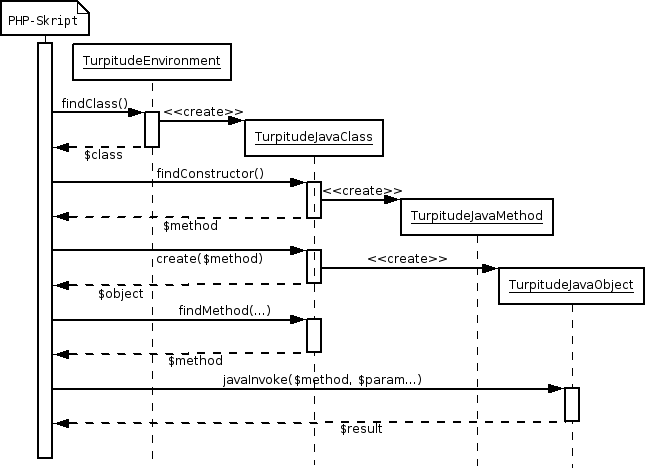
\includegraphics[width=\textwidth]{chap1/img/phpseq.png}
\caption{Ablauf eines PHP-Skriptes mit Zugriff auf Java-Objekte}
\label{fig:phpseq}
\end{figure}



% ********** End of chapter **********
